\newpage

\graphicspath{{main/hardware/graphics/}}

\subsection{Test Harness}

% present tense 

To accurately test the real time behaviour of the system, an external test harness is required. While latencies and jitter can be measured on-target with instrumentation, this does not independently measure the system's performance. Though this harness, an example control loop implementation can be simulated to ensure all deadlines are met during a live software update.

\begin{figure}[ht]
    \centering
    \begin{tikzpicture}  
        \node[block] (gen) {Signal\\Generator}; 
        \node[block, right=2cm of gen] (sw) {Software\\Infrastructure};
        \node[block, right=2cm of sw] (rcv) {Signal\\Receiver};  
        
        \node[block, text width=12cm, minimum height=1cm, below=1cm of sw] (har) {Harness}; 
        \node[block, minimum height=1cm, below=1cm of har] (ana) {Analyser};  

        \draw[->,thick] (gen) edge (sw);
        \draw[->,thick] (sw) edge (rcv);

        \draw[->,thick] (gen.south) edge ([xshift=-5.3cm]har.north);
        \draw[->,thick] (rcv.south) edge ([xshift=5.3cm]har.north);

        \draw[->,thick] (har) edge (ana);
    \end{tikzpicture}  
    \caption[Test Harness Design]
    {Test Harness Design}
    \label{fig:testHarnessDesign}
\end{figure}

\autoref{fig:testHarnessDesign} contains a signal generator, this randomly produces a signal and outputs a packet. These packets are ingested by the software infrastructure where processing occurs. An output packet is subsequently generated (mirroring the input) and sent to a signal receiver, which captures this packet.

The signal generator and receiver output their current state over discrete digital signals so that a logic analyser can record the state of the system over time. Specifically the states can be compared to measure the complete system latency during standard operation and software update. If the generator and receiver produce additional reference clock signals, the logic analyser can more closely calculate the software infrastructure induced latency.

\begin{figure}[ht]
    \centering
    \begin{tikztimingtable}[%
        timing/dslope=0.1,
        timing/.style={x=2ex,y=2ex},
        x=2ex,
        timing/rowdist=3ex,
    ]
        \busref{Generator Clock} & 2l 10{4c} \\
        \busref{Reciever Clock } & 11{4c} \\
        \busref{Generator Signal} & 6h 16l 16h 4l \\
        \busref{Reciever Signal} & 8h 16l 16h 4l \\

        \busref{Latency} & 6l D{} 14l  D{} 14l D{} 2l \\
        \extracode
            \begin{pgfonlayer}{background}
            \begin{scope}[semitransparent ,semithick]
                \vertlines[darkgray,dotted]{0.5,1.0 ,...,20.0}
            \end{scope}
        \end{pgfonlayer}
    \end{tikztimingtable}
    \caption[Test Harness Capture]
    {Test Harness Capture}
    \label{fig:testHarnessCapture}
\end{figure}

% start past tense

\begin{figure}[ht]
    \centering
    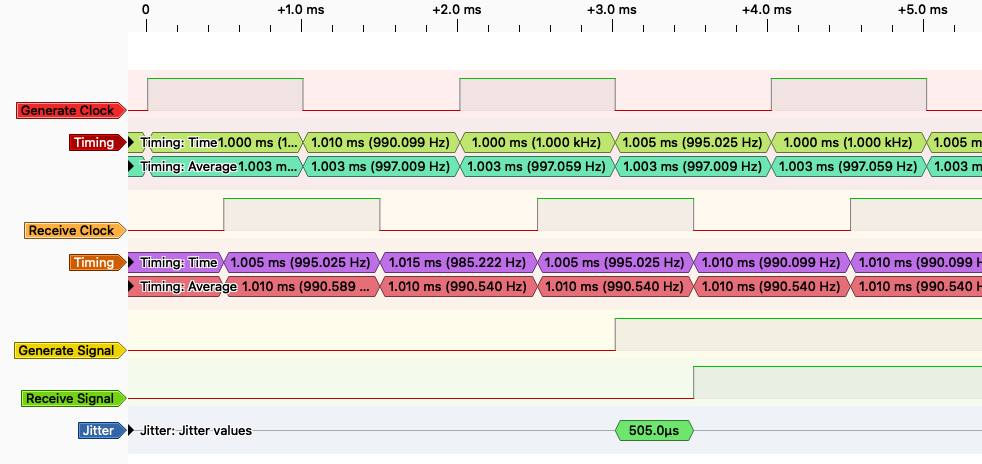
\includegraphics[width=\textwidth]{testHarnessPluseViewCapture.png}
    \caption[Test Harness PluseView Capture]
    {Test Harness PluseView Capture}
    \label{fig:testHarnessPluseViewCapture}
\end{figure}

The generator, receiver and logic analyser were all implemented using the RP2040 microprocessor from Raspberry Pi for hardware simplification. 

The two controllers that performed packet communication used the W5500 chip to send UDP packets over ethernet, this integrates nicely with Elafry messages. This co-processor offloads the complex ethernet drivers and communicates to the main proicessor over

% DIAGRAM - SPI block diagram

This communicates over SPI and offload sthe compelx ethernet stuff onto this co-processor. SPI signals confiure the IP address of the taregt device and allow the user to send data.

The intention for this software was to also use Rust, however we could not get the Rust libaries for the W5500 working quickly, sure with extra time with sould have been possible.
To simplify this software the arduino development environment was used. This as all the drivers for the w5500 are integrated in arduino libraries.

% DIAGRAM - ethernet diagram (with switch)

Logic analyser  
https://github.com/dotcypress/ula

Capture the status of the 16 input channels on the Pi Pico at specified frequencies.
When integrated with teh Pulseview analysis software we can idenitify the latencies  
